\documentclass[16pt,a4paper,oneside,titlepage]{report}
\usepackage[utf8]{inputenc}
\usepackage[UKenglish]{babel}
\usepackage{hyperref}
\usepackage[T1]{fontenc}
\usepackage{amsfonts}
\usepackage{lmodern}
\usepackage{amsmath}
\usepackage{amssymb}
\usepackage{mathrsfs}
\usepackage{graphicx}
\usepackage{subfig}
\usepackage[left=2cm,right=2cm,top=2cm,bottom=2cm]{geometry}
\author{Timé KADEL, Flavien REYNAUD}
\title{
 \textbf{Rapport de Travaux Pratiques}\\
 Simulation d'antennes imprimées\\
 \begin{figure}[h]
\center
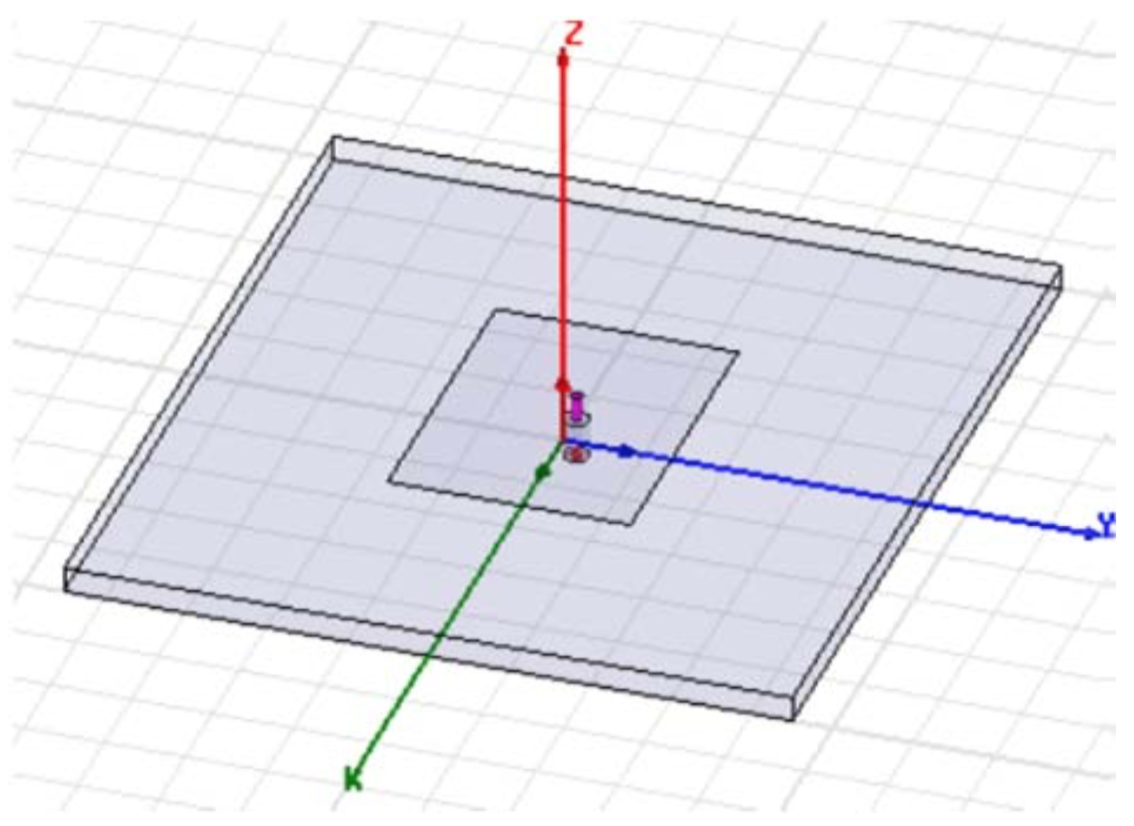
\includegraphics[scale=0.4]{Images/Titre.png}
\end{figure}
 }
\date{Octobre 2016}
\usepackage{fancyhdr}
\usepackage{lcd}
\usepackage[framemethod=tikz]{mdframed}
\pagestyle{fancy}
\usepackage{titlesec}
\usepackage{color}
\usepackage{layout}
\usepackage{longtable}
\usepackage{array}
\usepackage{appendix}
\usepackage{titlesec}
\usepackage{lipsum}
\usepackage{rotating}
\usepackage{tikz}
\usepackage{float}

\titleformat{\chapter}[display]
  {\normalfont\bfseries}{}{0pt}{\huge}

\renewcommand{\footrulewidth}{1pt}
\AtBeginDocument{\renewcommand{\bibname}{References}}
\fancyhead[L]{Simulation d'antennes imprimées}
\fancyhead[R]{Travaux Pratiques}
\fancyfoot[C]{\textbf{page \thepage}} 
\fancyfoot[L]{ESEO Angers}
\fancyfoot[R]{Octobre 2016}
\patchcmd{\chapter}{\thispagestyle{plain}}{\thispagestyle{fancy}}{}{}

\titlespacing*{\chapter}{0pt}{0pt}{40pt}

\long\def\chaptervc#1{\vfill\chapter{#1}\vfill\clearpage}

\let\EndItemize\enditemize
\def\enditemize{\EndItemize\bigskip}

\setcounter{secnumdepth}{3}
\setcounter{tocdepth}{4}

\begin{document}

\maketitle 
\tableofcontents
\listoffigures

\chapter{Introduction}

L'objectif de ces travaux pratiques est d'étudier des antennes imprimées de différentes formes et de comparer leurs caractéristiques électriques et leurs diagrammes de rayonnement.\\\\
Dans les deux premières parties, nous avons modélisé et simulé les antennes avec le logiciel ADS et analysé les résultats obtenus.\\\\
La dernière partie de ce rapport consiste en une simulation électromagnétique en 3D via le logiciel HFSS/Ansys.\\\\
Ce rapport se décompose en trois parties : 
\begin{itemize}
\item Conception d'une antenne microbande (patch)
\item Conception d'antenne demi-onde
\item Simulation électromagnétique en 3D
\end{itemize}

\chapter{Conception d'une antenne microbande (patch)}

L'objectif de ce chapitre est d'étudier et d'optimiser une antenne microbande fonctionnant à 2,4GHz sur un substrat en FR4.\\\\

\section{Premier cas}
Les données de cette partie sont les suivantes :\\\indent
$\epsilon_{r}=4,6 $\\\indent
$\sigma _{en}=5,7.10^7 S/m $\\\indent
$\tan\phi _{d}=\tan D=2.10^{-3} \rightarrow \phi _{d}\approx0,11 $\\\indent
$\mathcal{C}_{Cu} =17,8\mu m \rightarrow \:épaisseur \:de \:cuivre$\\\\
Afin de créer le masque, on doit préalablement calculer les dimensions de l'élément rayonnant repésenté ci-dessous :
\begin{figure}[h]
\center
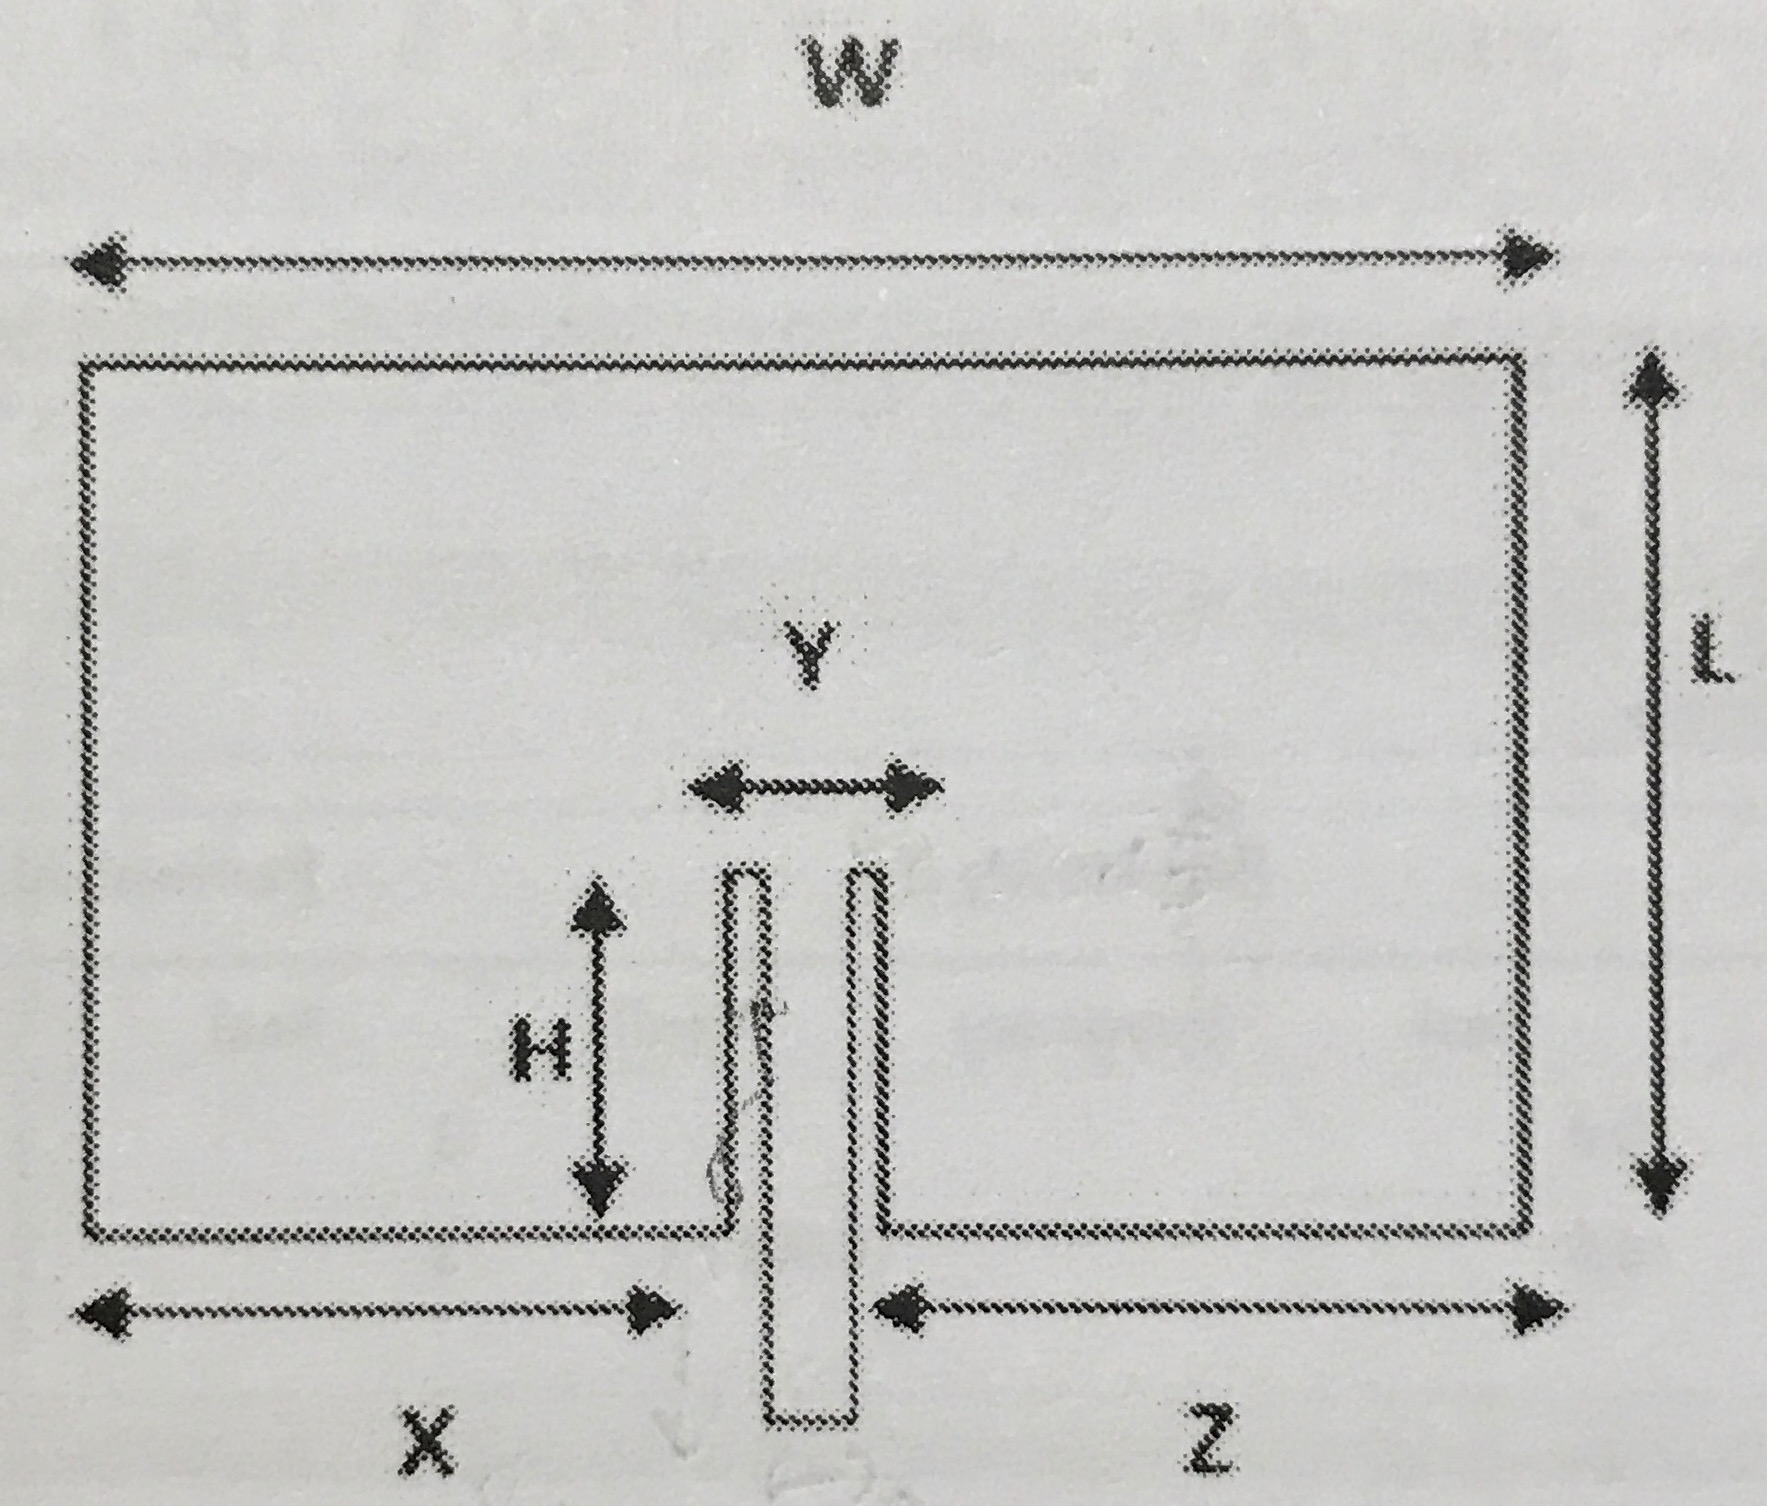
\includegraphics[scale=0.04]{Images/element_rayonnant.jpg}
\caption{Elément rayonnant}
\end{figure}

$W=L= \frac{v_{0}}{2f*\sqrt{\epsilon_{r}}}=29,14$\\\indent
$H= 0.822*\frac{L}{2}=11,977$\\\indent
$Y= \frac{W}{5}=5,83$\\\indent
$X=Z= \frac{2W}{5}=11,656$\\\indent
$X+Y+Z=W$\\\\

On crée le masque de l'élément rayonnant selon les coordonnées calculées précédemment. Le résultat est représenté sur la figure ci-après.
\begin{figure}[h]
\center
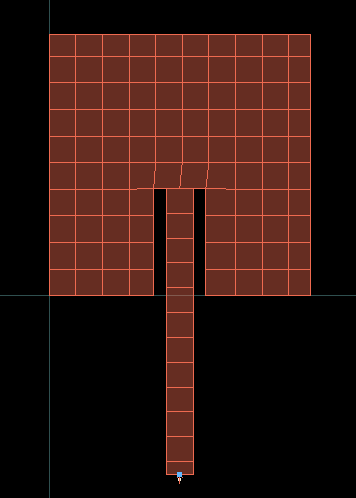
\includegraphics[scale=0.5]{Images/P3_Q2.png}
\caption{Création du masque de l'élément rayonnant}
\end{figure}

On place ensuite le port P1 au point d'alimentation de l'antenne, coordonnées (14,565;-20), comme représenté par la figure ci-dessous.
\begin{figure}[h]
\center
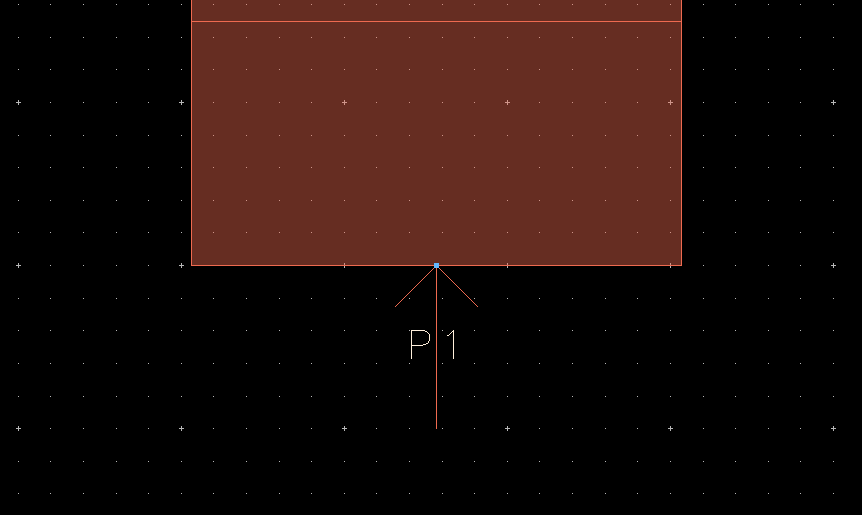
\includegraphics[scale=0.25]{Images/P3_Q3.png}
\caption{Placement diu port P1 au point d'alimentation de l'antenne}
\end{figure}

Après avoir définit la plage fréquentielle de simulation de 2,1GHz à 2,7GHz (balayage adaptatif), on simule et on obtient les résultats suivants :
\begin{figure}[h]
\center
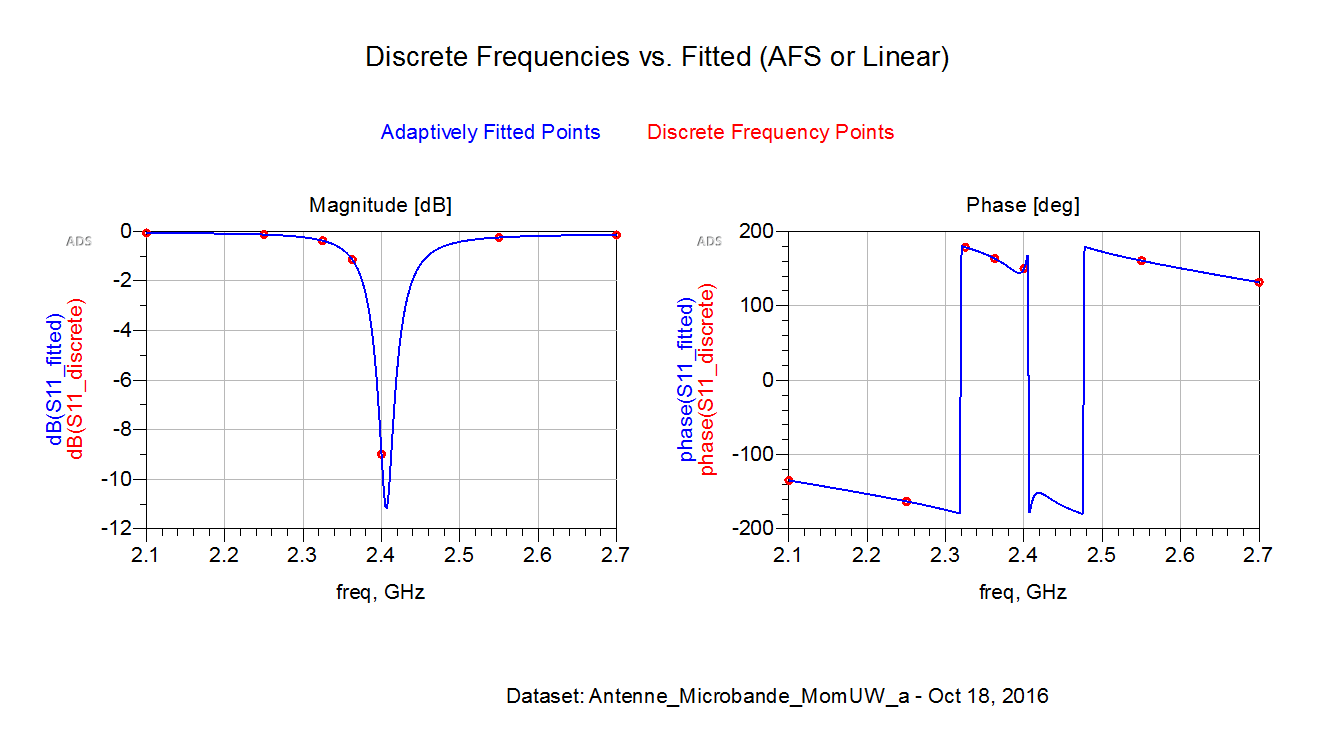
\includegraphics[scale=0.4]{Images/P3_Q6-1.png}
\caption{Discrete Frequencies vs Fitted (AFS or Linear)}
\end{figure}

Nous obtenons une adaptation de -11dB à 2,4GHz, ce qui est un résultat satisfaisant.\\\\
Calcul de la bande passante théorique :\\
$BW = 3,77*\frac{\epsilon -1}{\epsilon^2}*\frac{W}{L}*\frac{t}{\lambda}$\\\indent
$BW = 3,77*\frac{4,6 -1}{4,6^2}*\frac{29,14}{29,14}*1,6*\frac{2,4.10^9}{3.10^8}$\\\indent
$BW = 8MHz$\\\\
On a donc une bande passante théorique de 8MHz. \\
En pratique, on obtient une bande passante d'environ 10MHz.\\\\
Afin de déterminer la bande passante en pratique à -10dB, on place des marqueurs comme sur le graphique suivant :
\begin{figure}[h]
\center
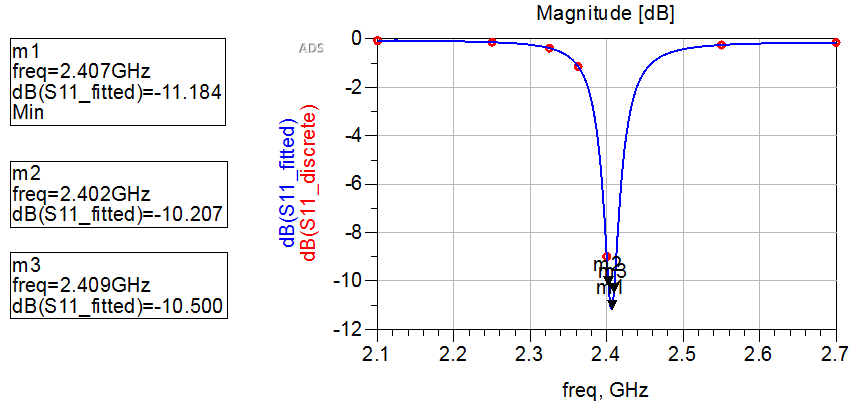
\includegraphics[scale=0.4]{Images/P3_Q7.png}
\caption{Discrete Frequencies vs Fitted (AFS or Linear)}
\end{figure}

On remarque qu'on obtient une bande passante d'environ 10MHz, ce qui correspond à la valeur théorique calculée. La différence s'explique en partie par l'approximation de placement des marqueurs. En effet, ADS ne permet pas de placer un pointeur avec une valeur précise.

Nous obtenons le diagramme de rayonnement en champ lointain suivant :
\begin{figure}[h]
\center
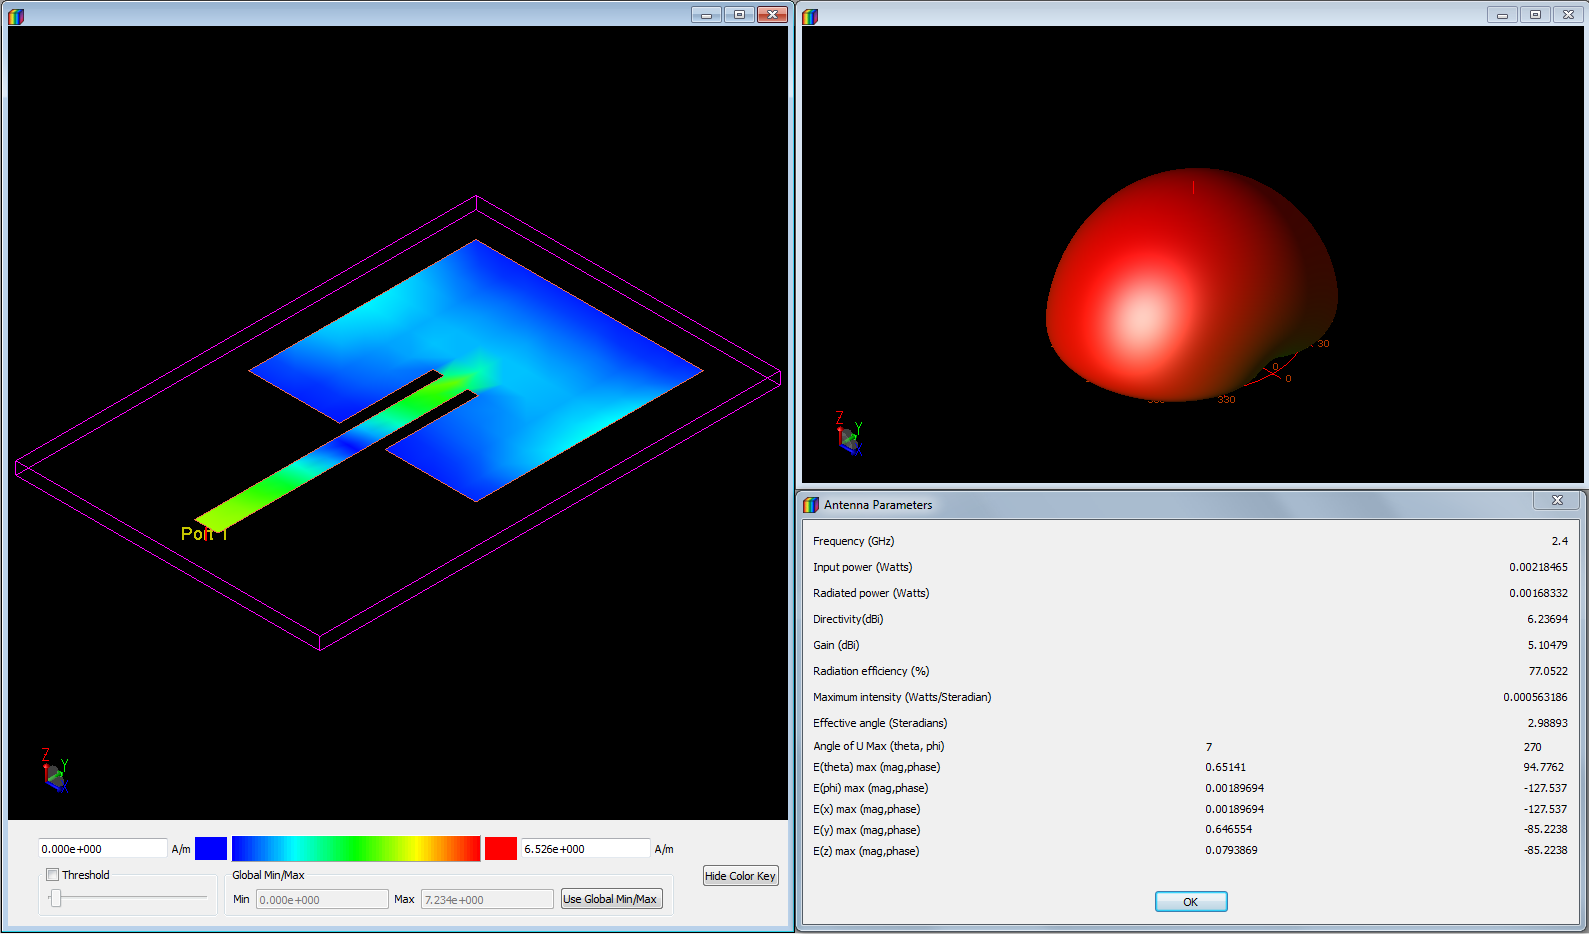
\includegraphics[scale=0.25]{Images/P3_Q8-ab.png}
\caption{Diagramme de rayonnement en champ lointain}
\end{figure}

Les paramètres selon phi et theta sont affichés sur la figure suivante :
\begin{figure}[h]
\center
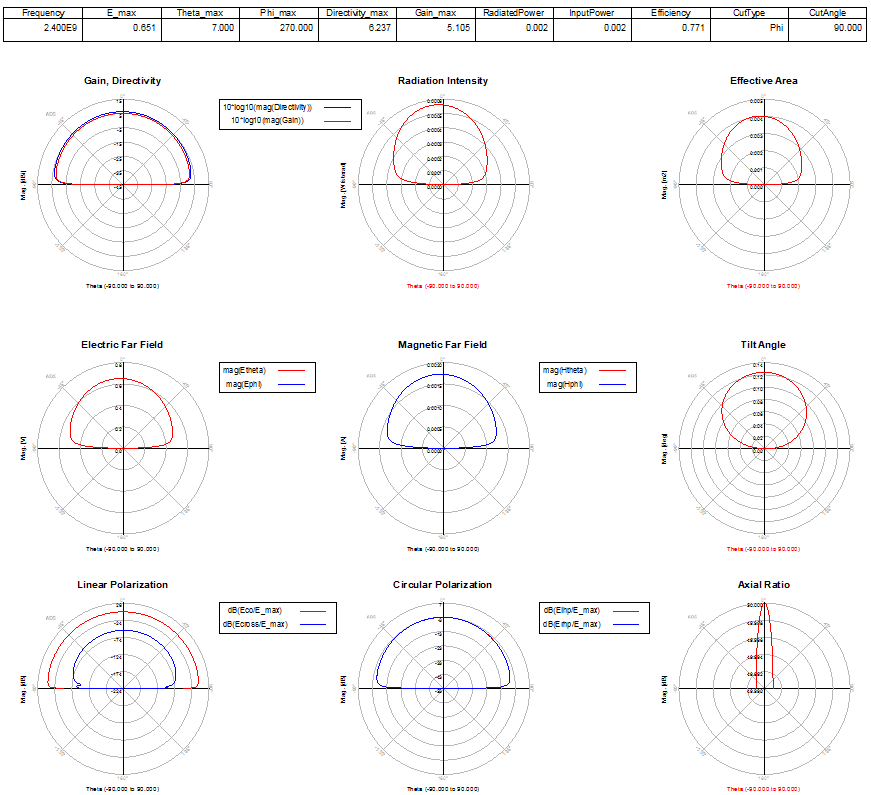
\includegraphics[scale=0.55]{Images/P3_Q8-cd.png}
\caption{Paramètres selon phi et theta en champ lointain}
\end{figure}

Le gain obtenu est de 5,1dBi et la directivité de 6,2dBi. \\
On note un rendement d'environ 70\% que nous allons améliorer en modifiant le design du masque.\\\\

\newpage
Nous avons dans un premier temps modifié notre masque de la manière suivante, afin d'obtenir une polarisation circulaire. 
\begin{figure}[h]
\center
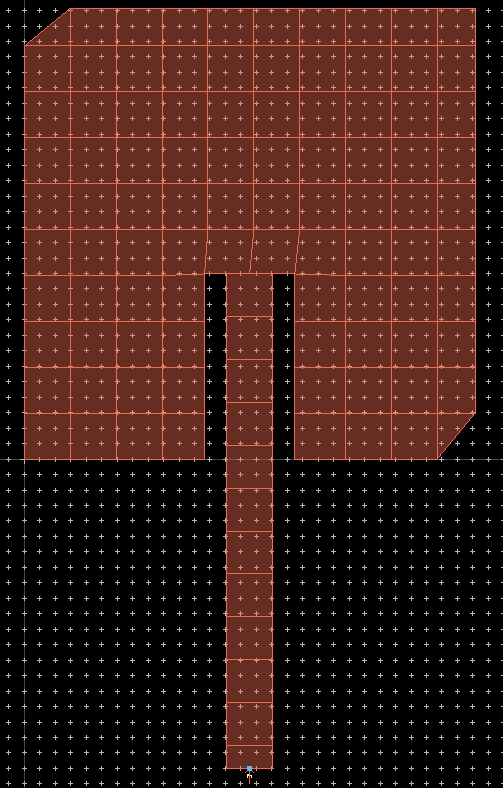
\includegraphics[scale=0.2]{Images/P3_Q9.png}
\caption{Masque modifié de l'élément rayonnant}
\end{figure}

En simulant, nous obtenons les courbes et diagramme de rayonnement suivants :
\begin{figure}[h]
\center
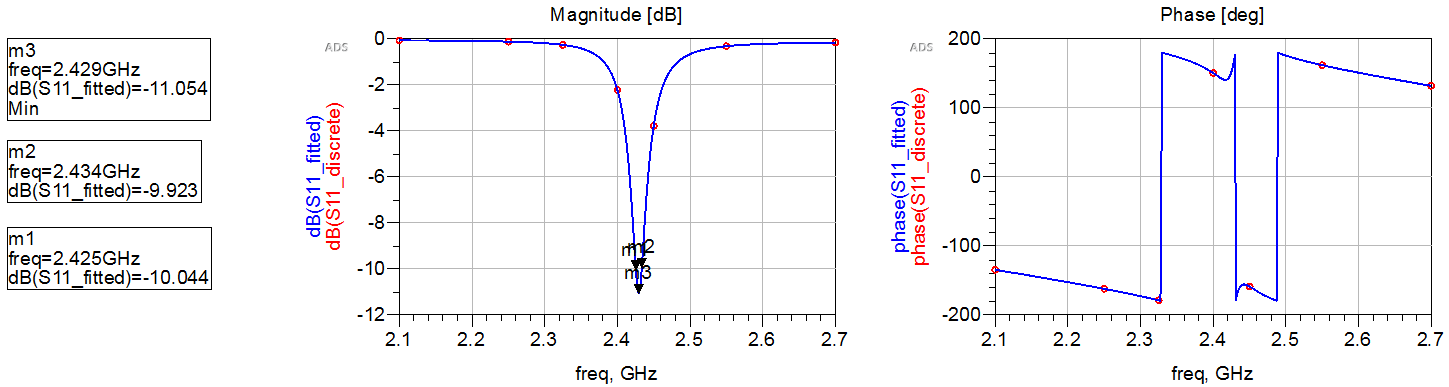
\includegraphics[scale=0.4]{Images/P3_Q9-1.png}
\caption{Discrete Frequencies vs Fitted (AFS or Linear)}
\end{figure}

\begin{figure}[h]
\center
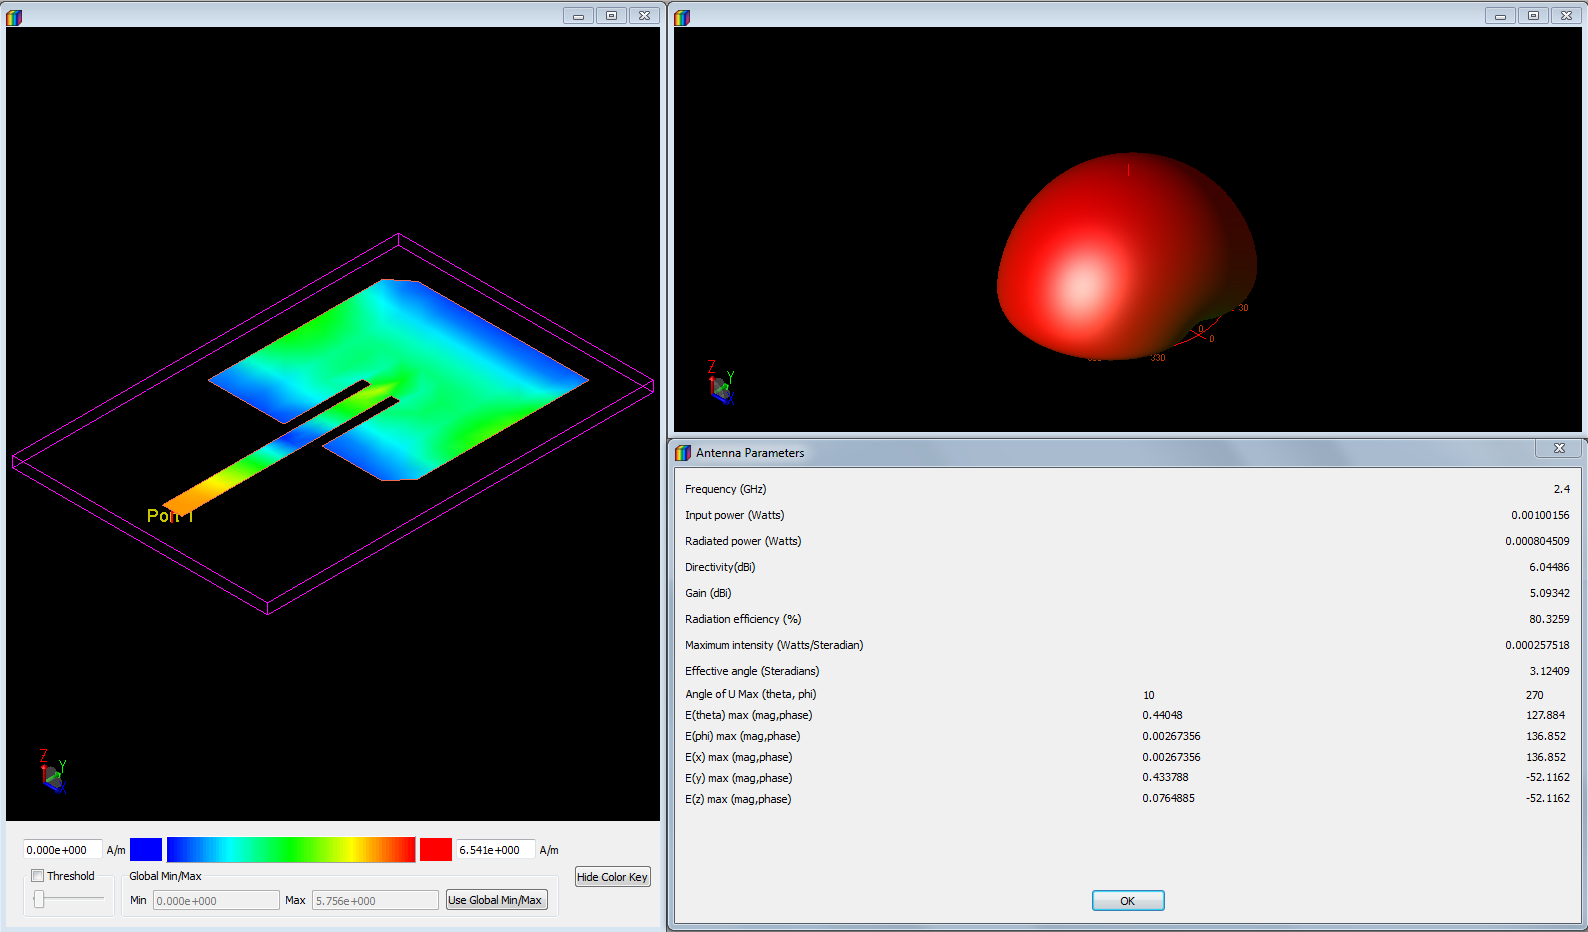
\includegraphics[scale=0.3]{Images/P3_Q9-2.png}
\caption{Diagramme de rayonnement en champ lointain}
\end{figure}

Le gain obtenu est de 5,1dBi et la directivité de 6,05dBi, ce qui reste quasiment inchangé par rapoort aux simulations précédentes. \\
On note cependant un rendement plus élevé, environ 80\%.\\\\
\newpage

Suite aux résultats précédents, nous décidons d'essayer d'améliorer encore le masque afin d'obtenir une meilleure polarisation circulaire. Après plusieurs essais et simulations, nous avons réussi a obtenir un masque ayant une polarisation circulaire assez bonne. Le masque est représenté sur la figure suivante.\\\\

\begin{figure}[h]
\center
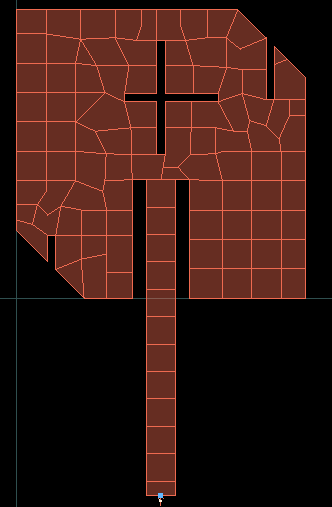
\includegraphics[scale=0.5]{Images/P3_Q9-BON.png}
\caption{Masque modifié de l'élément rayonnant}
\end{figure}

En simulant, nous obtenons les courbes et diagramme de rayonnement suivants :\\\\
\begin{figure}[h]
\center
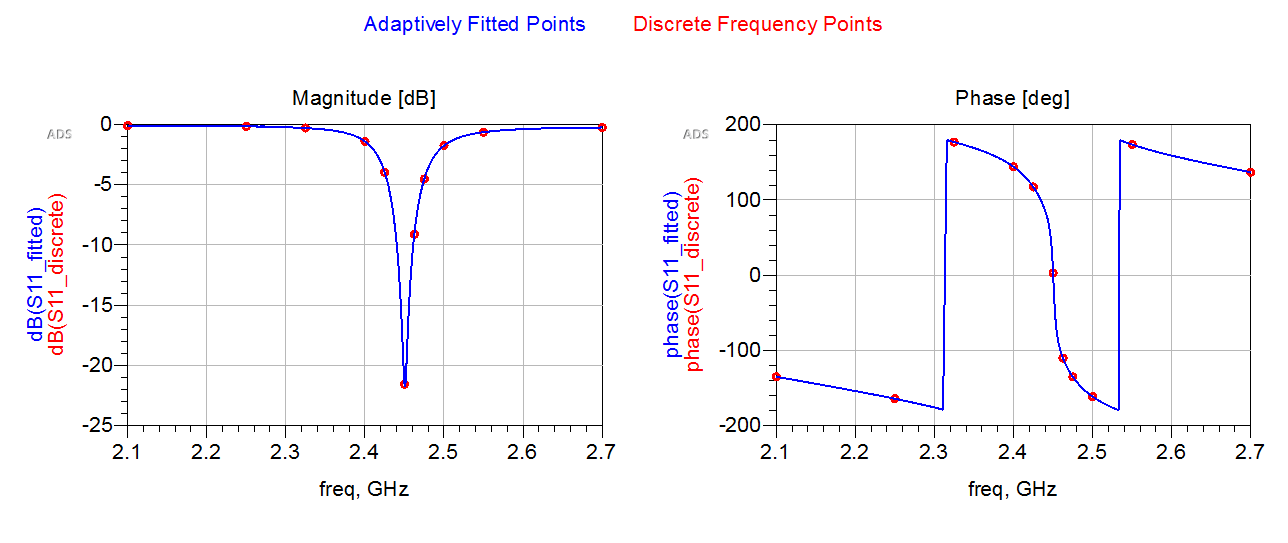
\includegraphics[scale=0.5]{Images/P3_Q9-BON3.png}
\caption{Discrete Frequencies vs Fitted (AFS or Linear)}
\end{figure}

\begin{figure}[h]
\center
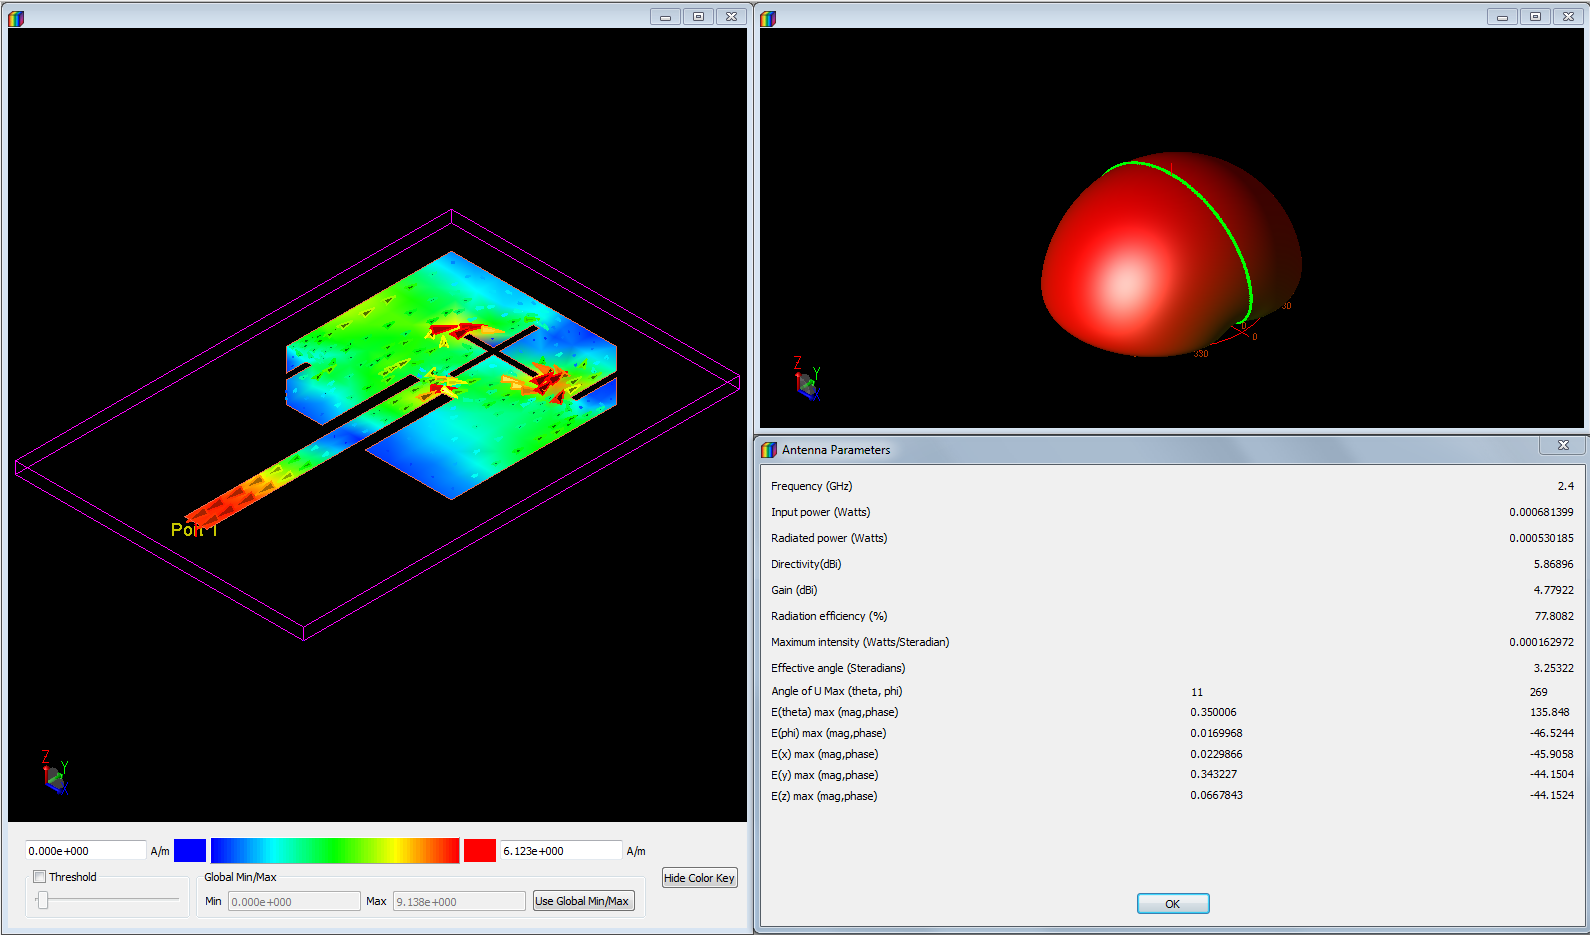
\includegraphics[scale=0.3]{Images/P3_Q9-BON1.png}
\caption{Diagramme de rayonnement en champ lointain}
\end{figure}

\begin{figure}[h]
\center
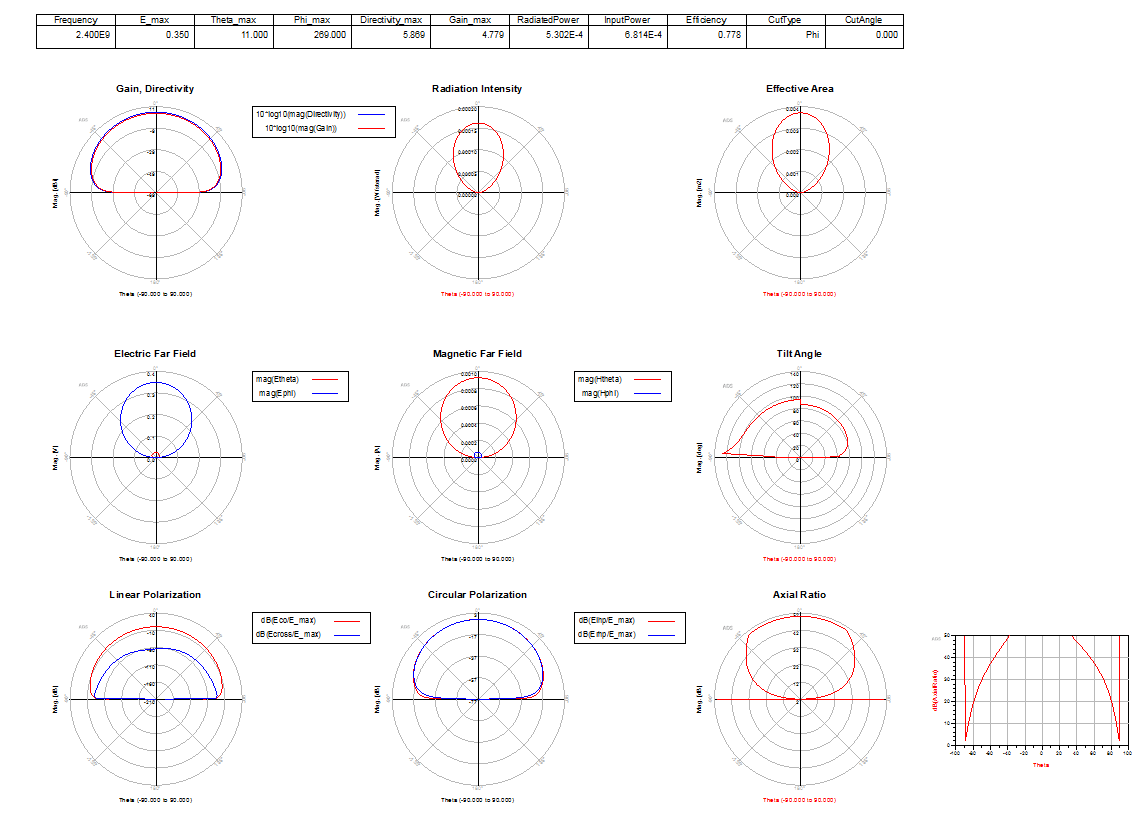
\includegraphics[scale=0.55]{Images/P3_Q9-BON2.png}
\caption{Paramètres selon phi et theta en champ lointain}
\end{figure}

\begin{figure}[h]
\center
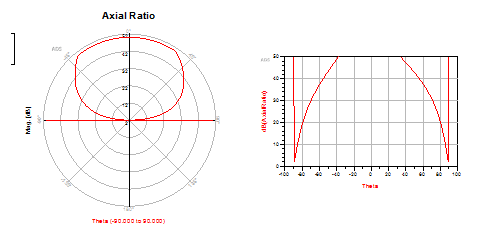
\includegraphics[scale=0.55]{Images/P3_Q9-BON22.png}
\caption{Axial ratio}
\end{figure}

Le gain obtenu est de 4,8dBi et la directivité de 5,9dBi, ce qui reste proche des simulations précédentes. \\
On note cependant un rendement plus élevé, environ 78\%.\\
On voit bien sur la figure 2.13 que la polarisation est circulaire, ce que nous cherchions à optimiser.\\\\



\clearpage
\section{Second cas}

On refait ensuite l'étude en changeant la valeur de l'épaisseur de cuivre : $\mathcal{C}_{Cu} =35\mu m$\\

En simulant, nous obtenons les courbes et diagramme de rayonnement suivants :
\begin{figure}[h]
\center
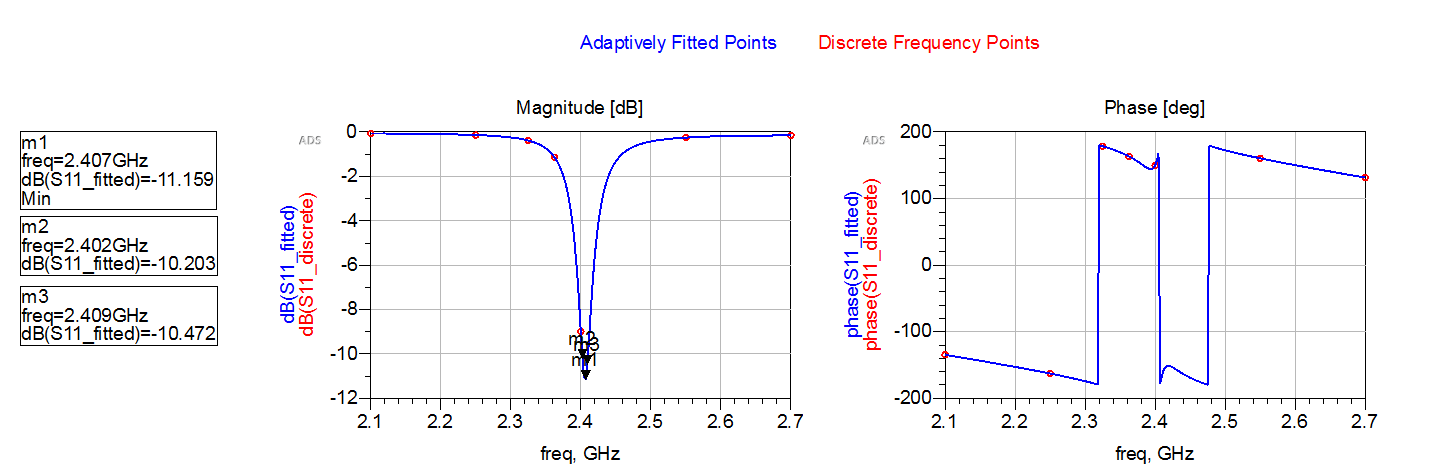
\includegraphics[scale=0.5]{Images/P3_Q10-1.png}
\caption{Discrete Frequencies vs Fitted (AFS or Linear)}
\end{figure}

\begin{figure}[h]
\center
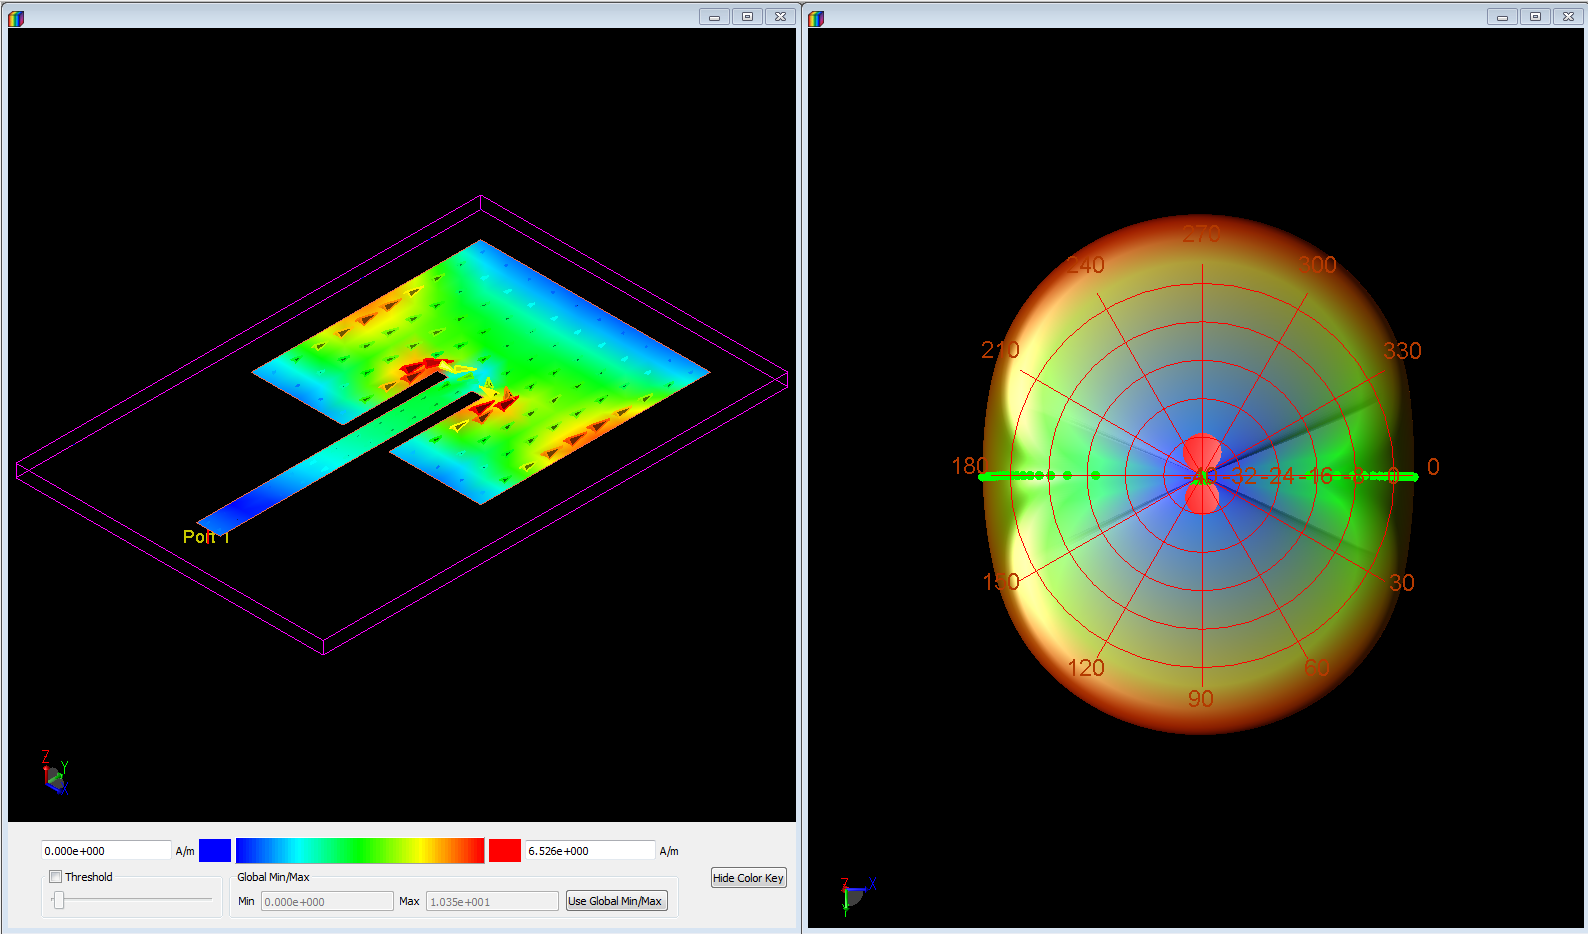
\includegraphics[scale=0.4]{Images/P3_Q10-2.png}
\caption{Diagramme de rayonnement}
\end{figure}

\clearpage
Nous changeons ensuite le substrat en choisissant le substrat Roger's de permitivité relative de 2,2.\\

En simulant, nous obtenons les courbes et diagramme de rayonnement suivants :
\begin{figure}[h]
\center
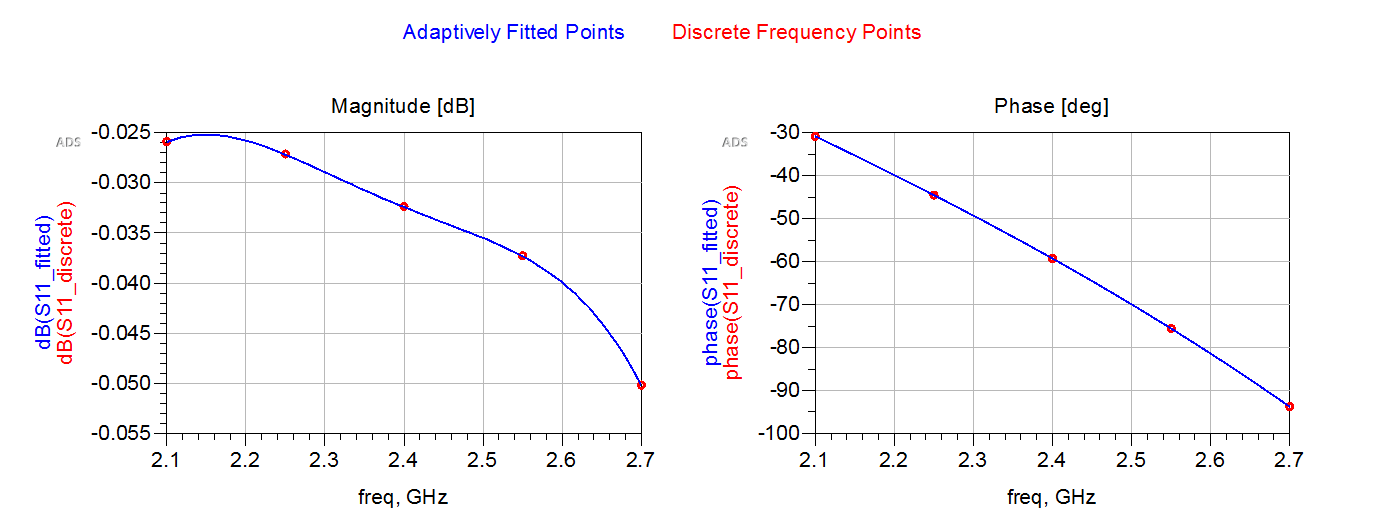
\includegraphics[scale=0.5]{Images/P3_Q11-1.png}
\caption{Discrete Frequencies vs Fitted (AFS or Linear)}
\end{figure}

Suite aux différentes simulations réalisées et à l'étude des différents résultats, nous pouvons en conclure que lorsqu'on diminue la permittivité, on concentre moins d'énergie, donc on augmente le rendement et par conséquent on augmente la fréquence. La fréquence est donc inversement proportionnelle à la permittivité.\\
De plus, lorsqu'on augmente la taille du substrat, on élargit la bande passante qui passe dans notre cas de -10dB à -8dB. 


\chapter{Conception d'antenne demi-onde}

Le but de ce chapitre est de réaliser et simuler une antenne planaire de longueur $\lambda/2$, fonctionnant à une fréquence de 1575,72 MHz pour des applications GPS. L'antenne doit être orientée selon l'axe Oz et alimentée en son centre par une tension de 1V.\\\\
 
On travaille en mode différentiel. La fréquence de la porteuse est de 1,57GHz et la longueur de l'antenne est de $\lambda/4$.
Nous avons besoin de produire un déphasage de 90 degrés pour que l'antenne résonne à la fréquence voulue. Pour ce faire, on utilise une longueur de 4,74cm.\\\\
Nous réalisons tout d'abord le schéma électrique équivalent de l'antenne. 

\begin{figure}[h]
\center
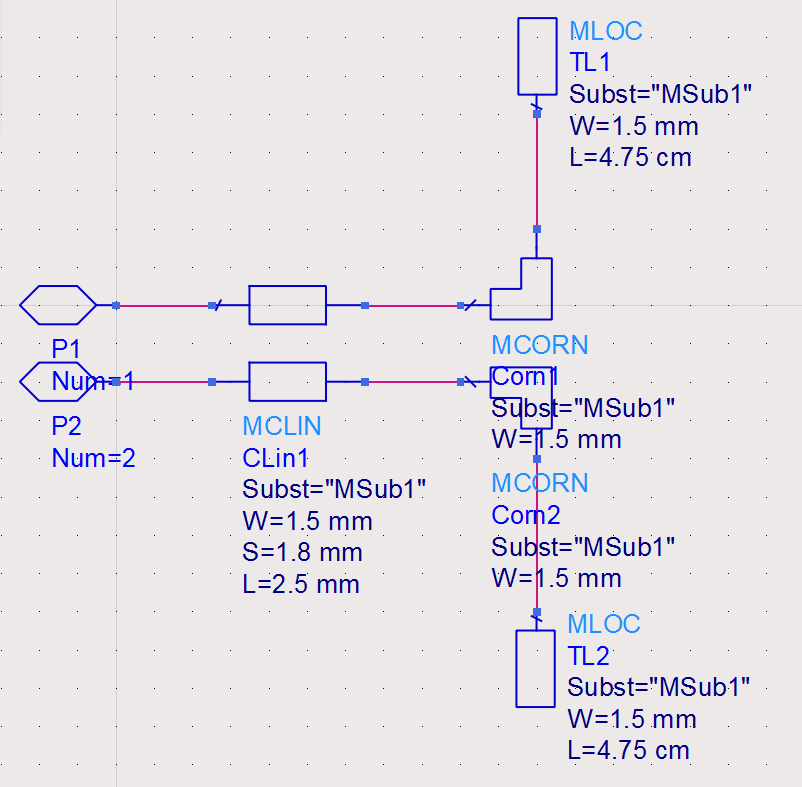
\includegraphics[scale=0.3]{Images/P1_Q1.png}
\caption{Schéma équivalent d'une antenne planaire de fréquence 1575,72 MHz}
\end{figure}

Nous générons ensuite son masque sous Momentum.\\\\

\begin{figure}[h]
\center
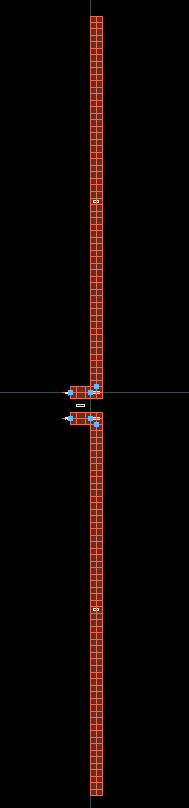
\includegraphics[scale=0.6]{Images/P1_Q2-1.png}
\caption{Masque de l'antenne planaire de fréquence 1575,72 MHz}
\end{figure}

\clearpage
Puis nous lançons la simulation en modèle électromagnétique.\\\\

\begin{figure}[h]
\center
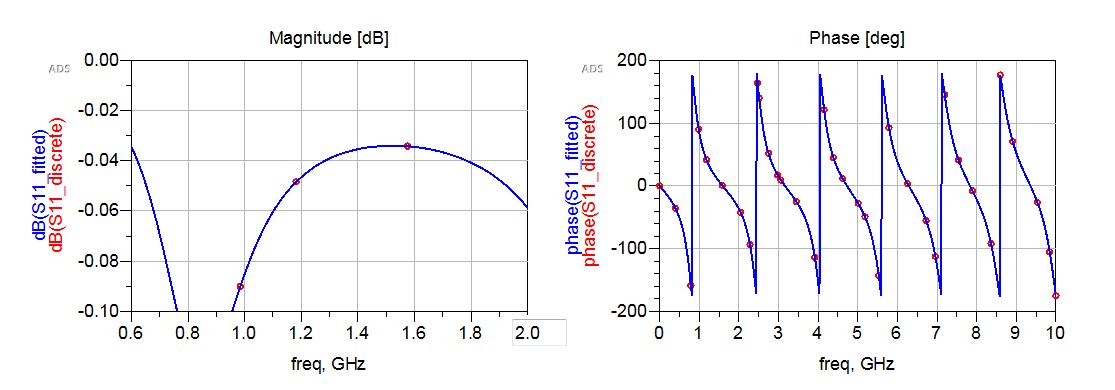
\includegraphics[scale=0.5]{Images/P1_Q2-2.png}
\caption{Courbes représentant la magnitude en dB et la phase en degrés - paramètre S(1,1)}
\end{figure}

\begin{figure}[h]
\center
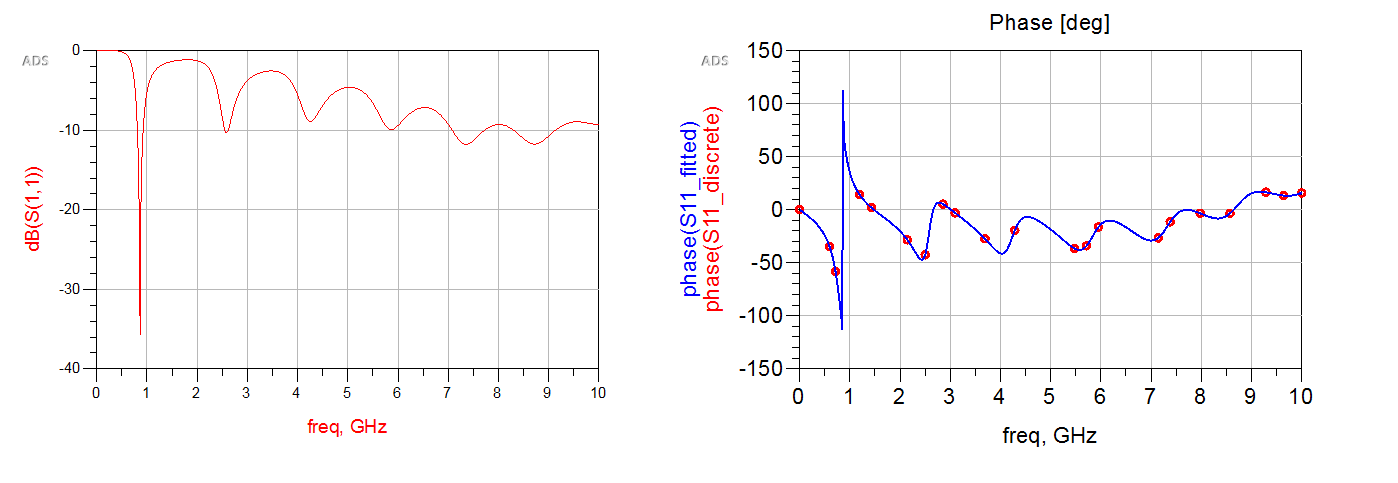
\includegraphics[scale=0.5]{Images/P1_Q2-3.png}
\caption{Courbes représentant la magnitude en dB et la phase en degrés - paramètre S(1,1)}
\end{figure}

D'après la courbe de la matrice S11, nous avons un pic à la fréquence de 0,9GHz où dB(S(1;1))=-13dB, ce qui est une bonne adaptation. 

\chapter{Conclusion}

Ces travaux pratiques nous ont permis de mieux comprendre le fonctionnement des antennes en réalisant et en étudiant différentes formes de masques, avec différents substrats, différentes dimensions, etc. 








\end{document}